\documentclass[12pt, letterpaper]{article}
\usepackage[colorlinks=true,linkcolor=black,citecolor=blue,filecolor=cyan,pagecolor=blue]{hyperref} 
\usepackage[toc,style=altlistgroup,hyperfirst=false]{glossaries}
\usepackage[utf8]{inputenc} %para poder escribir símbolos no anglosajones 
\usepackage[spanish, mexico]{babel} %Escribir en español (acentos)
\usepackage[T1]{fontenc}
\usepackage{amssymb}
\usepackage{mathtools}
\usepackage[usenames]{color}
\usepackage{float}
\usepackage{graphicx}  %%para las imagenes
\usepackage{cite} % para contraer referencias
\usepackage{multicol}
\usepackage{multirow}
\usepackage{bm}
\usepackage{bbm}
\usepackage[left=2.5cm,top=2.5cm,right=2.5cm,bottom=2.5cm]{geometry}
\parindent=5mm
\graphicspath{{images/}}
\usepackage{etoolbox}
\let\bbordermatrix\bordermatrix
%\patchcmd{\bbordermatrix}{8.75}{4.75}{}{}
%\patchcmd{\bbordermatrix}{\left(}{\left[}{}{}
%\patchcmd{\bbordermatrix}{\right)}{\right]}{}{}
%%%%glosario
\makeindex
%\makeglossaries
%\input{./glosario.tex}

%%%%%%%%%%%%%%%%%%%%%%%%%%%%%%%%%%%%%%%%%%%%%%%%%%%%%%%%%%%%%%%%%%%%%%%%%%%%%
%%NOTA IMPORTANTE:
%%Para relacionar el glosario.tex con este archivo
%%Es necesario abrir la terminal (Simbolo del sistema en windows)
%%Ir a la carpeta contenedora y escribir el siguiente comando:
%%makeindex -s PROYECTO_final.ist -t PROYECTO_final.glg -o PROYECTO_final.gls PROYECTO_final.glo
%%%%%%%%%%%%%%%%%%%%%%%%%%%%%%%%%%%%%%%%%%%%%%%%%%%%%%%%%%%%%%%%%%%%%%%%%%%%%

%%%% inicio del documento
\begin{document}

\thispagestyle{empty}

%%%%%%% portada

\thispagestyle{empty}

\begin{minipage}[c][0.1\textheight][c]{0.2\textwidth}
\begin{center}
    
\includegraphics[width=4cm, height=4cm]{cimat}
\end{center}
\end{minipage}
\begin{minipage}[c][0.1\textheight][t]{0.8\textwidth}
\begin{center}
    {\hspace{2cm}\scshape Centro de Investigación en Matemáticas}
    \vspace{-.5cm}
\end{center}
\hspace*{1.0cm} \rule[0mm]{0.9\textwidth}{0.8mm}
\hspace*{1.17cm}   \rule[4mm]{0.9\textwidth}{0.1mm}
    \vspace{-1cm}
\begin{center}
    { \hspace{2cm}\scshape  Unidad Monterrey}
\end{center}
\end{minipage}

\begin{minipage}[c][0.6\textheight][t]{0.2\textwidth}
\begin{center}
\hskip2pt
\vrule width2.5pt height10cm
        \hskip1mm
        \vrule width1pt height10cm \\ \vspace{2cm}
        
\includegraphics[height=4.5cm]{mty}
        \end{center}
\end{minipage}
\begin{minipage}[c][0.9\textheight][t]{0.65\textwidth}
  \begin{center}

	
    \vspace{3.2cm}
    
%%%% TITULO EN PORTADA

  \scshape Proyecto No. 1.\\ \normalsize
  
  \vspace{2cm}  
  
    
            
    Métodos multivariados de Análisis de Datos\\
    \vspace{1cm}   
    Filtro de spam personalizado.\\
    \vspace{1cm}   
    \vspace{1cm}   
    Ricardo Cruz Sánchez\\
    Rolando Corona Jiménez
    \vspace{.5cm}   
  \end{center}
  
\end{minipage}

%TABLA DE INDICES
\pagebreak
\tableofcontents

\cleardoublepage
%INTRODUCCIÓN
\pagebreak
\section{Introducción.}

Aplicación de modelos de clasificación para obtener un filtro (personalizado) para correos electrónicos spam.

\section{Análisis exploratorio.}

\subsection{Descripción del conjunto de datos.}

El conjunto de datos proviene de una serie de correos electrónicos del personal de la empresa HP. Los correos etiquetados como spam fueron proporcionados por el administrador del servidor de correo de la empresa, mientras que los correos que no están etiquetados como spam corresponden a correos personales y de trabajo de George Forman, es por ello que palabras como \textit{george} o código de área $650$ son indicadores de no spam. La base de datos fue creada por Mark Hopkins, Erik Reeber, George Forman y Jaap Suermondt de Hewlett-Packard Labs.

En total se cuentan 4601 observaciones, de las cuales 1813 fueron etiquetadas como spam, que corresponde al $39.4\%$ del total. Las observaciones están representadas a través de un conjunto de 58 atributos: $57$ variables cuantitativas y una variable cualitativa nominal de clase. Ninguno de los atributos presenta datos faltantes. 

\begin{table}[ht]
\centering
\begin{tabular}{|l|l|l|}
\hline
Spam     & $1813$ & $39.4 \%$ \\ \hline
Non-Spam & $2788$ & $60.6 \%$ \\ \hline
\end{tabular}
\caption{Distribución de clases.}
\label{t_dist}
\end{table}

\subsection{Diccionario de datos}

Los 58 atributos se pueden agrupar en:

\begin{itemize}
	\item 48 variables cuantitativas continuas con rango $[0,100]$, de la forma word\_freq\_WORD, que indica el porcentaje de palabras en el correo que coinciden con WORD, es decir:
	$$word\_freq\_WORD = 100 \times \dfrac{\#\text{apariciones de WORD en el correo}}{\#\text{total de palabras en el correo}}$$
	
	\item 6 variables cuantitativas continuas con rango $[0,100]$, de la forma char\_freq\_CHAR, que indica el porcentaje de caracteres en el correo que coinciden con CHAR, es decir:	
		$$char\_freq\_CHAR = 100 \times \dfrac{\#\text{apariciones de CHAR en el correo}}{\#\text{total de caracteres en el correo}}$$
		
	\item 1 variable cuantitativa continua \textsf{capital\_run\_length\_average} con rango $[0,\infty)$, que es igual a longitud media de las secuencias contiguas de letras mayúsculas que aparecen en el correo.
	
	\item 1 variable cuantitativa discreta \textsf{capital\_run\_length\_longest} con rango $[0,\infty)$, que es igual a la longitud de la secuencia contigua de letras mayúsculas más larga que aparece en el correo.
	
	\item 1 variable cuantitativa discreta \textsf{capital\_run\_length\_total} con rango $[0,\infty)$, que es igual a la suma de las longitudes de las secuencias contiguas de letras mayúsculas que aparecen en el correo.
	
	\item 1 variable nominal de clase con valores en $\{0, 1\}$, que indica si el correo se considera spam (1) o no (0).
\end{itemize}

La documentación del conjunto de datos no indica los criterios para la selección de las 48 palabras y 6 caracteres usados para la definición de sus correspondientes variables.

\begin{table}[ht]
\centering
\begin{tabular}{|l|l|l|l|l|l|}
\hline
make     & order     & business & hp     & data       & cs         \\ \hline
address  & mail      & email    & hpl    & 415        & meeting    \\ \hline
all      & receive   & you      & george & 85         & original   \\ \hline
3d       & will      & credit   & 650    & technology & project    \\ \hline
our      & people    & your     & lab    & 1999       & re         \\ \hline
over     & report    & font     & labs   & parts      & edu        \\ \hline
remove   & addresses & 000      & telnet & pm         & table      \\ \hline
internet & free      & money    & 857    & direct     & conference \\ \hline
\end{tabular}
\caption{Palabras que corresponden a las variables de tipo word\_freq\_WORD.}
\label{t_words}
\end{table}

\begin{table}[ht]
\centering
\begin{tabular}{|l|}
\hline
;   \\ \hline
(   \\ \hline
{[} \\ \hline
!   \\ \hline
\$  \\ \hline
\#  \\ \hline
\end{tabular}
\caption{Caracteres que corresponden a las variables de tipo char\_freq\_CHAR.}
\label{t_chars}
\end{table}

\subsection{Matriz de correlación.}

\subsection{Palabras más frecuentes por clase.}

A modo de resumen se muestra una representación gráfica de las palabras más frecuentes por cada clase, para obtener la frecuencia de cada palabra, se realizó la suma de cada variable sobre todas las observaciones de cada clase.

\section{Métricas para clasificación binaria.}

Las métricas de evaluación permiten medir y resumir la calidad de un modelo entrenado al ser probado con nuevas observaciones. La exactitud ($accuracy$) es una de las métricas más comunes para evaluar la capacidad de generalización de un clasificador, sin embargo no siempre resulta ser la ideal, y esto depende específicamente del problema en cuestión. Entre la distintas métricas que existen para el problema de clasificación binaria, a continuación se mencionan algunas, para finalmente discutir sobre cuál es la ideal para la clasificación de spam, con el fin de tener un criterio de preferencia entre los clasificadores que serán presentados más adelante. \\

Existen dos tipos de errores al asignar una clase a una observación: el \textit{falso positivo} $fp$ (diagnóstico positivo, condición de interés ausente) y el \textit{falso negativo} $fn$(diagnóstico negativo, condición de interés presente). De forma similar se definen los verdaderos positivos $tp$ y verdaderos negativos $tn$. \\

A partir de lo anterior, se definen las métricas de interés que se muestran en la tabla \ref{t_metricas}.

\begin{table}[ht]
\centering
\begin{tabular}{|l|l|l|}
\hline
\textbf{Métrica} & \textbf{Fórmula}             & \textbf{Enfoque de la evaluación}                \\ \hline
Accuracy         & $\dfrac{tp+tn}{tp+fn+fp+tn}$ & Desempeño general                                \\ \hline
Sensitivity      & $\dfrac{tp}{tp+fn}$          & Efectividad para identificar a la clase positiva \\ \hline
Specificity      & $\dfrac{tn}{fp+tn}$          & Efectividad para identificar a la clase negativa \\ \hline
\end{tabular}
\caption{Métricas para clasificación binaria}
\label{t_metricas}
\end{table}

\subsection{Selección de métricas para el problema del spam.}

Para la clasificación de spam, es fundamental que los correos que no son spam, en la medida de lo posible, no sea etiquetados como spam, pues de lo contrario, los usuarios podrían perder información de valor si no revisan periódicamente la bandeja de spam, lo cual sería contraproducente. Dicho en términos de las métricas mencionadas anteriormente, se desea un clasificador con alta especificidad (specificity), de modo que la probabilidad de que un correo que no es spam no sea marcado como spam, sea alta. Sin embargo, puede pasar que al aumentar la especificidad, la exactitud y la sensibilidad (sensitivity) se vean reducidas, lo que causaría que el clasificador no se capaz de identificar muchos correos que deberían ser marcados como spam, en cuyo caso el usuario los recibiría en su bandeja principal y tendría que marcar manualmente dichos correos como spam. Este último enfoque es preferido, pues se trata de garantizar que los usuarios no pierdan información de valor. Teniendo en cuenta estas consideraciones, se procede a ajustar una serie de clasificadores binarios.


\section{Modelos de clasificación.}

\subsection{Regresión logística.}

\subsection{Máquinas de soporte vectorial.}

\subsection{Árboles de decisión.}

El índice de Gini se define como 

$$ G $$ 

gini
podado
matriz de costo

%o bagging
\subsection{Random Forest.}

\subsection{Modelos con reducción de dimensión y selección de variables}

\subsection{Representación en componentes principales.}

Se calculan las componentes principales y se grafica el screeplot, que muestra el porcentaje de varianza acumulada en función del número de componentes principales. La figura \ref{screeplot} muestra que, por ejemplo para explicar el $80\%$ de varianza, se requieren de al menos $30$ componentes principales, 
lo que sugiere que los modelos entrenados en dimensión reducida pueden tener un ajuste deficiente.

\begin{figure}[h]
\centering
	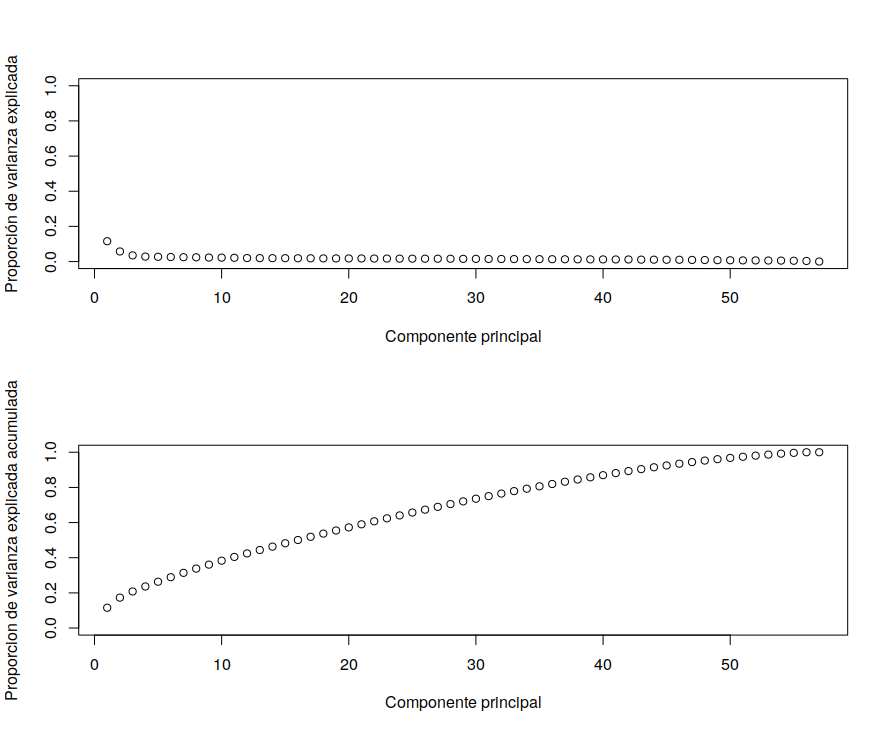
\includegraphics[scale=.5]{images/pca.png} 
	\caption{Screeplot}
		\label{screeplot}
\end{figure}


\subsection{Comparativa con otros modelos}

%provenientes de articulos
de spambase.DOCUMENTATION
$~7\%$ misclassification error.
False positives (marking good mail as spam) are very undesirable.
If we insist on zero false positives in the training/testing set,
$20-25\%$ of the spam passed through the filter.

revisar papers donde trabajan con el ejemplo

\section{Conclusiones.}


\begin{thebibliography}{1}

\bibitem{cr98}
Lorrie Faith Cranor and Brian A. LaMacchia. 1998. Spam!. Commun. ACM 41, 8 (August 1998), 74-83. 

\bibitem{fe19}
Emilio Ferrara. 2019. The history of digital spam. Commun. ACM 62, 8 (July 2019), 82-91. 

\bibitem{ha01}
Hastie, T., Tibshirani, R.,, Friedman, J. (2001). The Elements of Statistical Learning. New York, NY, USA: Springer New York Inc.. 

\bibitem{so09}
Marina Sokolova and Guy Lapalme. 2009. A systematic analysis of performance measures for classification tasks. Inf. Process. Manage. 45, 4 (July 2009), 427-437. 

\end{thebibliography}

\end{document}